
\section{Attitude Parameterization of Rigid Bodies}

The matrix $\textbf{T}_{IB}$ is a 3x3 transformation matrix that
rotates a vector from the body to the inertial frame. A transformation
matrix has the unique property that the inverse of the transformation
is just the transpose of the matrix. There are multiple ways to
construct this rotation frame and a few ways are discussed in the
sections that follow. 

\subsection{Euler Angles}\label{s:Euler_Angles}

Euler angle are used to describe 3 unique rotation from the inertial
to body frame. They are typically denoted as $\psi$, $\theta$ and
$\phi$. The order of the rotation can vary however the 3-2-1 sequence
is standard for aircraft while the 3-1-3 sequence is standard for
spacecraft. 

\subsubsection{3-2-1 Sequence}

The transformation from the inertial frame to the body frame involves
three unique rotations. The first is a rotation about the z-axis such
that
\begin{equation}
{\bf C}_A(\vec{v}_{C/I}) = [{\bf T}_{IA}]^T{\bf C}_I(\vec{v}_{C/I})= \begin{bmatrix} cos(\psi) & sin(\psi) & 0
  \\ -sin(\psi) & cos(\psi) & 0 \\ 0 & 0 & 1 \end{bmatrix} {\bf C}_I(\vec{v}_{C/I})
\end{equation}
this rotation is called the yaw or heading rotation. Note that the matrix $[{\bf T_{IA}}]$ is a matrix that rotates a vector from the A frame to the inertial frame. The transpose of this matrix rotates a vector from the inertial frame to the A frame. From here the
intermediate frame (A frame) is rotated about the y-axis such that
\begin{equation}
{\bf C}_{NR}(\vec{v}_{C/I}) = [{\bf T}_{ANR}]^T{\bf C}_A(\vec{v}_{C/I})=\begin{bmatrix} cos(\theta) & 0 &
  -sin(\theta) \\ 0 & 1 & 0 \\ sin(\theta) & 0 & cos(\theta) \end{bmatrix} {\bf C}_A(\vec{v}_{C/I})
\end{equation}
this rotation is called the pitch angle rotation. Finally the (NR) no roll
frame is rotated through the x-axis such that
\begin{equation}
{\bf C}_{B}(\vec{v}_{C/I}) = [{\bf T}_{NRB}]^T{\bf C}_{NR}(\vec{v}_{C/I})=\begin{bmatrix} 1 & 0 & 0 \\ 0 & cos(\phi) & sin(\phi)
  \\ 0 & -sin(\phi) & cos(\phi) \end{bmatrix} {\bf C}_{NR}(\vec{v}_{C/I})
\end{equation}
A Figure of this is shown below.
\begin{figure}[H]
  \begin{center}
  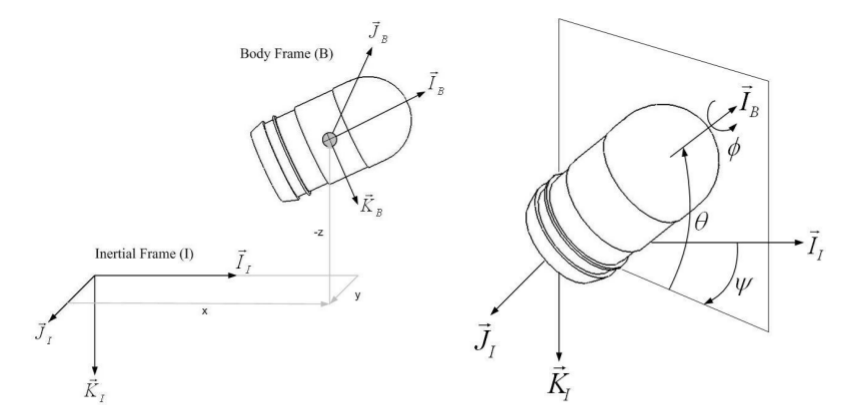
\includegraphics[height=50mm, width=120mm]{Figures/6DOFrocketschematic.png}
  \end{center}
  \caption{Six Degree of Freedom Schematic}
\end{figure}
Putting all of these 2-D rotations together creates a
transformation matrix from body to inertial. 
\begin{equation}
{\bf C}_{B}(\vec{v}_{C/I}) = [{\bf T}_{NRB}]^T[{\bf T}_{ANR}]^T[{\bf T}_{IA}]^T{\bf C}_{I}(\vec{v}_{C/I}) = [{\bf T}_{IB}]^T{\bf C}_{I}(\vec{v}_{C/I})
\end{equation}
Note again that the inverse of this matrix is given below using the properties of matrix transposes. Standard shorthand
notation is used for trigonometric functions: $ cos(\alpha) \equiv
c_{\alpha} $ , $ sin(\alpha) \equiv s_{\alpha} $ , and $ tan(\alpha)
\equiv t_{\alpha} $.
\begin{equation}\label{e:TIB}
{\bf T}_{IB}(\phi,\theta,\psi) = {\bf T}_{IA}{\bf T}_{ANR}{\bf T}_{NRB}=\begin{bmatrix} c_{\theta}c_{\psi} &
s_{\phi}s_{\theta}c_{\psi}-c_{\phi}s_{\psi} &
c_{\phi}s_{\theta}c_{\psi} + s_{\phi}s_{\psi} \\ c_{\theta}s_{\psi} &
s_{\phi}s_{\theta}s_{\psi} + c_{\phi}c_{\psi} &
c_{\phi}s_{\theta}s_{\psi} - s_{\phi}c_{\psi} \\
-s_{\theta} & s_{\phi}c_{\theta} & c_{\phi}c_{\theta}
\end{bmatrix}
\end{equation}

\subsubsection{Derivatives}

If Euler angles are used to parameterize the orientation, the
derivative of Euler angles is somewhat cumbersome to obtain. The angular
velocity of a body is typically written as
\begin{equation}
\vec{\omega}_{B/I} = \begin{Bmatrix} p \\ q
  \\ r \end{Bmatrix} = p \hat{I}_B + q \hat{J}_B + r \hat{K}_B
\end{equation}
There are no inertial components for the angular velocity
vector. However, a relationship can be derived relating the
derivatives of the Euler angles. The angular velocity can be written
in vector form such that
\begin{equation}
\vec{\omega}_{B/I} = \dot{\psi} \hat{K}_I + \dot{\theta} \hat{J}_{NR} +
\dot{\phi} \hat{I}_B
\end{equation}
relating the unit vectors $\hat{K}_I$ and $\hat{J}_{NR}$ to the body
frame using the planar rotation matrices results in the equation
below. Note that NR is denoted as the ``No-Roll" frame.
\begin{equation}\label{e:ptpdot}
\begin{Bmatrix} \dot{\phi} \\ \dot{\theta} \\ \dot{\psi} \end{Bmatrix}
= [\textbf{H}]
\begin{Bmatrix} p\\q\\r\end{Bmatrix}
\end{equation}
where
\begin{equation}
\textbf{H}=\begin{bmatrix} 1 & s_{\phi}t_{\theta} & c_{\phi}t_{\theta} \\ 0 &
c_{\phi} & -s_{\phi} \\ 0 & s_{\phi}/c_{\theta} &
c_{\phi}/c_{\theta} \end{bmatrix}
\end{equation}

\subsubsection{Screw Rotation}

It is often useful to extract Euler Angles from a unit vector. A unit
vector has two degrees of freedom and thus has two rotations
$\psi$ and $\theta$ which can be determined using the
equation below where $\hat{n}(1)$ denotes the first component of
the vector in the body frame. 
\begin{equation}
  \psi = tan^{-1}\left ( \frac{\hat{n}(2)}{\hat{n}(1)}
  \right) ; \\
  \theta_{Ri} = tan^{-1} \left ( \frac{\hat{n}(3)}{\hat{n}(1)^2 + \hat{n}(2)^2}
  \right)
\end{equation}

\subsubsection{Transformation Matrix to Euler Angles}

Besides using unit vectors, sometimes it is beneficial to extract
Euler angles from a known tranformation matrix. The equations below
can be used to accomplish this where ${\bf T}_{BI}(i,j)$ is the ith row and
jth column of the ${\bf T}_{BI}$ matrix where ${\bf T}_{BI} = {\bf T}_{IB}^T$
\begin{equation}
  \begin{matrix}
  \theta = -sin^{-1}({\bf T}_{BI}(1,3)) & \phi =
  tan^{-1}({\bf T}_{BI}(2,3)/{\bf T}_{BI}(3,3)) & \psi =
  tan^{-1}({\bf T}_{BI}(1,2)/{\bf T}_{BI}(1,1)) \end{matrix}
\end{equation}

\subsection{Quaternions}\label{s:quat}

\subsubsection{The General Quaternion}

It is well known that equations of motion produced by using only three
orientation parameters results in a singularity \cite{etkins}. As
such, the orientation of the vehicle can be parameterized using four
parameters known as quaternions. Many supplemental equations and
explanations can be found for quaternions in
\cite{Lin,Filipe,multibody,quaternions,cassidis,Munoz,Markley,Liu_Estimation}. I
also recommend visiting an interactive visualization tool made by
popular YouTube star Ben Eater \url{https://eater.net/quaternions}. To
begin, The standard quaternion is written below.
\begin{equation}
  \vec{q} = \begin{Bmatrix} q_0 \\ q_1 \\ q_2 \\ q_3 \end{Bmatrix}
\end{equation}
In this case 4 parameters are used to denote the quaternion. In order
to get a physical understanding of what a quaternion is imagine a
vector $\vec{\eta}$ in 3-D space. The rotation from the body to the
inertial frame is then the rotation of the inertial frame about the
unit vector $\vec{\eta}$ through angle $\gamma$. The quaternion can
then be written as
\begin{equation}
  \vec{q} = \begin{Bmatrix} cos(\gamma/2)
    \\ \vec{\eta}sin(\gamma/2) \end{Bmatrix}
\end{equation}
In this case it is possible to obtain the individual quaterions as
$q_0 = cos(\gamma/2)$ and $\vec{\epsilon} = [q_1,q_2,q_3]^T =
\vec{\eta}sin(\gamma/2)$. Furthermore, if given 4 quaternions, the
angle $\gamma$ is simply $cos^{-1}(2q_0)$ and
$\vec{\eta}=\vec{\epsilon}/sin(\gamma/2)$. Note that because a quaternion is
essentially screw rotation about a known unit vector, there are two
identical quaternions for every orientation. That is $\vec{q}(\gamma) = \vec{q}(\gamma-2\pi)$.

\subsubsection{Quaternion Transformations}

In order to rotate the inertial frame to the
body frame using quaternions, the transformation matrix is shown
below. Note that ${\bf T}_{BI}={\bf T}_{IB}^T$. 
\begin{equation}
  {\bf T}_{BI}(\vec{q}) = \begin{bmatrix}
    {q_0}^2 + {q_1}^2 - {q_2}^2 - {q_3}^2 && 2(q_1q_2+q_0q_3) && 2(q_1q_3-q_0q_2)\\
    2(q_1q_2-q_0q_3) && {q_0}^2 - {q_1}^2 + {q_2}^2 - {q_3}^2 && 2(q_0q_1+q_2q_3)\\
    2(q_0q_2+q_1q_3) && 2(q_2q_3-q_0q_1) && {q_0}^2 - {q_1}^2 - {q_2}^2 + {q_3}^2
  \end{bmatrix}
\end{equation}

\subsubsection{Euler to Quaternion Transformations}

In the event Euler angles are need, converting quaternions to Euler
angles is a standard operation and shown below.
\begin{equation}
  \begin{matrix}
    \phi = tan^{-1}\left(\frac{2(q_0q_1 + q_2q_3)}{1-2(q_1^2 + q_2^2)}\right) \\
    \theta = sin^{-1}\left(2(q_0q_2-q_3q_1)\right) \\
    \psi = tan^{-1}\left(\frac{2(q_0q_3 + q_1q_2)}{1-2(q_2^2 +
      q_3^2)}\right)
  \end{matrix}
\end{equation}
It is also possible to convert Euler angles to quaternions using the
equations below.
\begin{equation}
  \begin{matrix}
    q_0 = cos(\phi/2)cos(\theta/2)cos(\psi/2) + sin(\phi/2)sin(\theta/2)sin(\psi/2)\\
    q_1 = sin(\phi/2)cos(\theta/2)cos(\psi/2) - cos(\phi/2)sin(\theta/2)sin(\psi/2)\\
    q_2 = cos(\phi/2)sin(\theta/2)cos(\psi/2) + sin(\phi/2)cos(\theta/2)sin(\psi/2)\\
    q_3 = cos(\phi/2)cos(\theta/2)sin(\psi/2) - sin(\phi/2)sin(\theta/2)cos(\psi/2)\\
  \end{matrix}
\end{equation}

\subsubsection{Quaternion Operations}

The norm of the quaternions is given by $|\vec{q}| =
\sqrt{q_0^2+q_1^2+q_2^2+q_3^2}$. In standard spacecraft applications,
the norm of the quaternion is just 1. The conjugate of the quaternion
$\vec{q}$ is given below.
\begin{equation}
  \vec{q}^{*} = \begin{Bmatrix} q_0 \\ -q_1 \\ -q_2  \\ -q_3 \end{Bmatrix}
\end{equation}
The inverse of a quaternion is then just $\vec{q}^{-1} = \vec{q}^* /
|\vec{q}|$. Determining the difference between two quaternions is done
using the quaternion difference operation as shown below where
$|\tilde{q}|=1.0$ \cite{quaternions}.
\begin{equation}\label{e:quat_difference}
  \delta \vec{q} = \vec{q}~\Earth~\tilde{q}^{-1} = \begin{Bmatrix}
    q_0\tilde{q}_0 - \vec{\epsilon}^T\tilde{\epsilon}
    \\ -q_0\tilde{\epsilon} + \tilde{q}_0\vec{\epsilon}-{\bf
      S}(\vec{\epsilon})\tilde{\epsilon} \end{Bmatrix}
\end{equation}

\subsubsection{Quaternion Derivatives}

The derivatives of a quaternion are written in shorthand using the
equation below. 
\begin{equation}
  \dot{\vec{q}} = \frac{1}{2}{\bf \Omega}(\vec{\omega}_{B/I})\vec{q} =
  \frac{1}{2}{\bf \chi}(\vec{q})\vec{\omega}_{B/I}
\end{equation}
The operators ${\bf \Omega}()$ and ${\bf \chi}()$ are shown below. Note that
${\bf \Omega}()$ operates on a $3 \times 1$ vector and ${\bf \chi}$ on a $4 \times 1$ vector.
In this case $\lambda = [\lambda_0,\vec{\kappa}]^T$.
\begin{equation}
  {\bf \Omega}(\vec{r}) = \begin{bmatrix} 0_{1x1} & -\vec{r}^T \\ \vec{r} &
    -{\bf S}(\vec{r})\end{bmatrix}
\end{equation}
\begin{equation}
  {\bf \chi}(\vec{\lambda}) = \begin{bmatrix} -\vec{\kappa}
    \\ \lambda_0I_{3x3} + {\bf S}(\vec{\kappa}) \end{bmatrix}
\end{equation}
These vector operators can then be used to expand the kinematic
derivatives as shown by equation \ref{e:quat}.
\begin{equation}\label{e:quat}
  \begin{Bmatrix} \dot{q}_{0} \\ \dot{q}_{1} \\ \dot{q}_{2}
    \\ \dot{q}_{3} \end{Bmatrix} = \frac{1}{2} \begin{bmatrix} 0 & -p & -q & -r
    \\ p & 0 & r & -q \\ q & -r & 0 & p \\ r & q & -p & 0 \end{bmatrix} \begin{Bmatrix} q_{0}
    \\ q_{1} \\ q_{2} \\ q_{3} \end{Bmatrix}
\end{equation}
where $q_{i}$ are the four quaternions and $p,q,~r$ are the components
of the angular velocity vector in the body frame.
